\chapter{Method}
\label{ch:proposedMethod}
In this chapter, we outline our approach for measuring the level of disagreement between various saliency-based methods. Firstly, we explain the mathematical formula behind four metrics that we used, which include feature agreement, sign agreement, rank correlation (inherited and adapted for images from \cite{krishna_disagreement_problem}), and structural similarity index metric. Next, we select several saliency-based methods for generating explanations, including both gradient-based and perturbation-based. We also discuss the selection of two black box convolutional neural networks (CNNs) - InceptionV3 and ResNet - and provide an overview of their architecture.

\section{Overview}
\label{sec:methodOverview}
Figure \ref{fig:methodOverview} summarizes our procedure for quantifying the disagreement between different saliency explanation methods. Initially, we train each targeted black box on the selected dataset that consists of x-ray images and matching masks. The specifics of this dataset will be discussed in depth in chapter \ref{ch:experimentsAndResult}. Subsequently, we apply the attribution algorithm of the chosen explanation methods to the test set, which generates an explanation for the black box per each test example. We then calculate the level of disagreement by using disagreement metrics for each pair of explanations per test example and aggregate the outcomes to create a comparison heatmap. Finally, we examine the heatmaps to determine whether there is any significant disagreement.

\begin{figure}
    \centering
    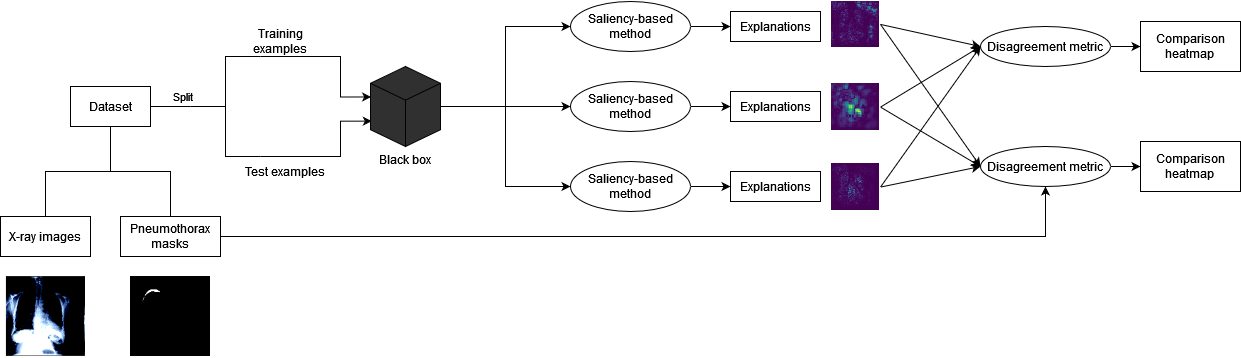
\includegraphics[width=\textwidth]{images/method-overview.png}
    \caption{An overview of the steps we've taken to quantify the disagreement between the explanation methods. These steps are applied per black box.}
    \label{fig:methodOverview}
\end{figure}

Note that this procedure is applied per black box. In our experiments in chapter \ref{ch:experimentsAndResult}, we applied this procedure to two different black boxes and analyzed the outcomes for both of them.
\section{Mathematical Formulation}
In this section, we establish certain mathematical notations that will be utilized to clarify the disagreement metrics.

\subsection{Saliency Maps}
For a given black box $b$ and a test instance $x$, where $x$ is an image of size $n \times n$, and an explanation method $c$, the saliency map explanation $e \in \mathbb{R}^{n\times n}$ for the black box $b$ with respect to test instance $x$ is obtained by running the attribution algorithm provided by $c$:
\begin{equation}
    e = c(b, x)
\end{equation}
Each value $e_{ij}$ represents the importance score that the pixel at $(i, j)$ contribute to the prediction of the black box $b$ at instance $x$. The range of values of $e_{ij}$ depends on the nature of the explanation method $c$.

\subsection{Metrics}
\label{subsec:metrics}
\subsubsection{Structural Similarity Index Metric}
To capture the similarity in structure between two saliency maps, we use the Structural Similarity Index Metric (SSIM) \cite{ssim}. Despite its name, this metric captures more than just structural similarity between two images: it takes into account the contrast, luminance, and the structure of two images.

For the sake of simplicity, given two saliency maps $e^{(1)}$ and $e^{(2)}$, let $x = e^{(1)}$, $y = e^{(2)}$. Then, the formula for SSIM between two saliency maps $x$ and $y$ is:
\begin{equation}
    \text{SSIM}(x, y) = [l(x, y)]^\alpha [c(x, y)]^\beta [s(x, y)]^\gamma
\end{equation}
where $l(x,y)$, $c(x,y)$, and $s(x,y)$ is the comparison of the luminance, contrast, and structure of two images $x$ and $y$, respectively; $\alpha$, $\beta$, and $\gamma$ are constansts that control the importance of the $l(x,y)$, $c(x,y)$, and $s(x,y)$, respectively.

Next, we present the definition of the three components of the SSIM. Let $\mu_x$, $\mu_y$ be the mean value of the saliency map $x$ and $y$; $\sigma_x$, $\sigma_y$ be the standard deviation of the $x$ and $y$; $\sigma_{xy}$ be the covariance of $x$ and $y$; $C_1$, $C_2$ and $C_3$ be small constants.

The luminance component is defined:
\begin{equation}
    l(x,y) = \frac{2\mu_x\mu_y + C_1}{\mu_x^2 + \mu_y^2 + C_1}
\end{equation}

Next, the contrast component is defined as:
\begin{equation}
    c(x,y) = \frac{2\sigma_x\sigma_y + C_2}{\sigma_x^2 + \sigma_y^2 + C_2}
\end{equation}

Finally, the structure component is defined as:
\begin{equation}
    s(x,y) = \frac{\sigma_{xy} + C_3}{\sigma_x\sigma_y + C_3}
\end{equation}

The constants $C_1$, $C_2$ and $C_3$ are typically set to small values in order to avoid zero division. $\alpha$, $\beta$ and $\gamma$ are usually set to 1, but they can be assigned with other values to emphasize or deemphasize their respective components.

In this work, because each saliency map differs in the range of its pixel values, we decided to measure SSIM using the magnitude of the saliency maps, normalized into the range $[0, 1]$ for fair comparison.

\subsubsection{Feature Agreement}
We utilize the feature agreement introduced by \cite{krishna_disagreement_problem}, adapted for images. For a saliency map $e$, a pixel $(i, j)$ is within the top-$k$ feature for $e$ if $|e_{ij}|$ is among the set of top-$k$ absolute values of all pixels of $e$. We denote the set of top-$k$ pixels of $e$ with $\text{top}_{k}(e)$. Then given two saliency map $e^{(1)}$ and $e^{(2)}$, the feature agreement between two maps is given by:

\begin{equation}
    \text{FA}_k(e^{(1)}, e^{(2)}) = \frac{|\text{top}_{k}(e^{(1)}) \cap \text{top}_{k}(e^{(2)})|}{k}
\end{equation}

Note that the above metric is equivalent to the following transformation and operation:
\begin{itemize}
    \item Taking the absolute value of both saliency maps
    \item Convert both saliency maps into a binary map in which pixels within top-$k$ are assigned the value 1, otherwise assigned the value 0
    \item The feature agreement of two saliency maps is computed by taking the size of the intersection of the 1s region and dividing by $k$
\end{itemize}

This metric captures how much the region that the two saliency maps consider most important overlaps with each other. Figure \ref{fig:featureAgreementDemo} presents the procedure to compute the feature agreement of a pair of explanations generated from Guided Backpropagation and Integrated Gradients. The feature agreement captures how much the two technique agrees for the top-5\% most salient pixels (for a $128\times128$ image, this is equivalent to $k= 820$).

\begin{figure}
    \centering
    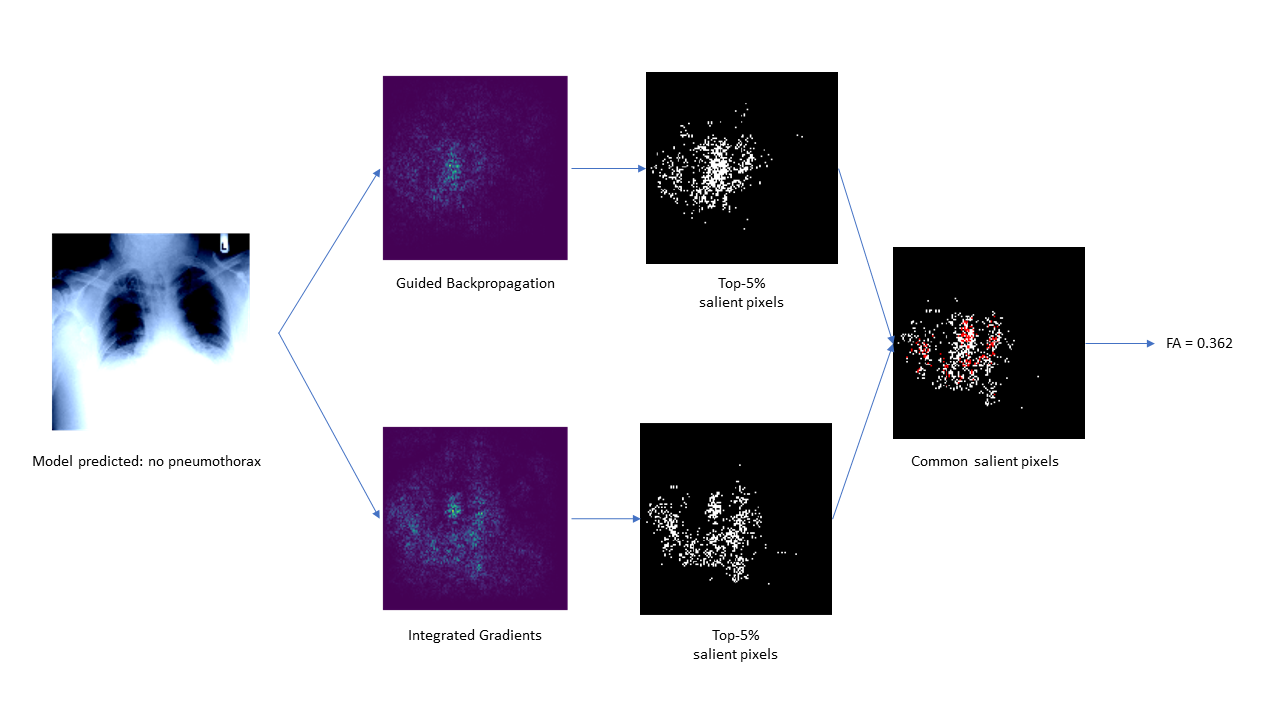
\includegraphics[width=\textwidth]{images/feature-agreement-demo.png}
    \caption{Illustration of how feature agreement was measured for an example pair of saliency maps generated by Guided Backpropagation and Integrated Gradients. We are interested in the top 5\% of the most important pixels ($k=820$ in total, colored white). The feature agreement score is calculated by determining the number of common top salient pixels (highlighted in red) and dividing this by $k$.}
    \label{fig:featureAgreementDemo}
\end{figure}


\subsubsection{Sign Agreement}
The sign agreement is quite similar to feature agreement, however, it is a stricter criterion \cite{krishna_disagreement_problem}. The sign agreement between two saliency maps $e^{(1)}$ and $e^{(2)}$ with respect to the top-$k$ features is:
\begin{equation}
    \text{SA}_k(e^{(1)}, e^{(2)}) = \frac{|\{(i, j) | (i, j) \in \text{top}_{k}(e^{(1)}) \cap \text{top}_{k}(e^{(2)}) \land e^{(1)}_{ij} \cdot e^{(2)}_{ij} > 0\}|}{k}
\end{equation}

The metric considers two saliency maps agree on a pixel if it is both significant in the two maps and has the same direction of contribution (negative or positive).

\subsubsection{Rank Correlation}
Another metric we adopted from the work of Krishna et al. \cite{krishna_disagreement_problem} is the rank correlation metric. In the original work, the metric is computed using the rankings of a subset of the input features. This feature subset when adapted to saliency maps can be represented as a mask. For any given matrix real matrix $d$ of size $m \times n$ (a saliency map can also be viewed as a matrix), a mask $m$ is a binary matrix of the same size, and the operation $m(d)$ return the set of $d_{ij}$ correspond to where $m_{ij} = 1$, that is:
\begin{equation}
    m(d) = \{d_{ij} | m_{ij} = 1, \forall i \in [1, m], \forall j \in [1, n]\}
\end{equation}

Given a saliency map $e$, we define $\text{rank}(e)$ to be the matrix of the rank of the pixel values of $e$. Then the rank correlation for two saliency maps $e^{(1)}$ and $e^{(2)}$ with respect to a mask $m$ is given by:
\begin{equation}
    \text{RC}(e^{(1)}, e^{(2)}, m) = r_s\left(m(\text{rank}(e^{(1)})), m(\text{rank}(e^{(2)}))\right)
\end{equation}
\section{Experiment Subjects}
\label{sec:experimentSubjects}

\subsection{Explanation Methods}
\label{subsec:explanationMethods}
We use the following saliency methods for our experiments: Occlusion as the single perturbation-based method, seven gradient-based methods including Vanilla Gradient or Saliency, GradientSHAP, Guided Backpropagation, Guided GradCAM, Integrated Gradients, DeepLift, and LRP. Specific hyperparameters were required for some of these methods, which we specified as follows:
\begin{itemize}
    \item For Occlusion: we use an $8\times8$ occlusion window and a $4\times4$ stride.
    \item For Integrated Gradients and GradientSHAP: we use a baseline generated from a uniform distribution on the interval $[0, 1)$.
\end{itemize}

\subsection{Black boxes}
We opted to use XAI methods on the InceptionV3 \cite{inceptionv3} and Resnet101 \cite{resnet101} architectures for several reasons. One primary reason is that these models are based on Convolutional Neural Networks (CNNs), which are necessary for certain model-specific XAI techniques like Class Activation Mapping (CAM) and Grad-CAM. These techniques leverage the inherent structure and characteristics of CNNs to produce visual explanations and highlight significant regions in an image. Additionally, we chose InceptionV3 and Resnet101 because of their demonstrated performance in previous work conducted by Narin, Ali et al. in their study on COVID-19 detection using X-ray images \cite{covidXray}. Although these models do not have sustainable G-ops (giga operations per second), they have shown good performance in specific applications, particularly in the medical domain. By applying XAI methods to these architectures, we aim to gain a deeper understanding of their performance in medical imaging tasks.

\subsubsection{Residual Network - 101}
\label{subsubsec:resnet101}
ResNet-101 is a convolutional neural network architecture that was introduced by He et al. in 2015 \cite{resnet101}. The residual network was developed to address the challenge of training very deep neural networks by utilizing residual connections.

The key idea of residual networks lies in their residual block design, which allows for the effective training of extremely deep models. In traditional deep networks, the increasing depth often leads to performance degradation due to the difficulty of learning mappings from input to output. A residual network solves this issue by introducing skip connections, or shortcut connections, that allow the network to learn residual mappings. By propagating gradients through these shortcuts, the model can effectively capture residual information and learn more efficiently.

\begin{figure}
\centering
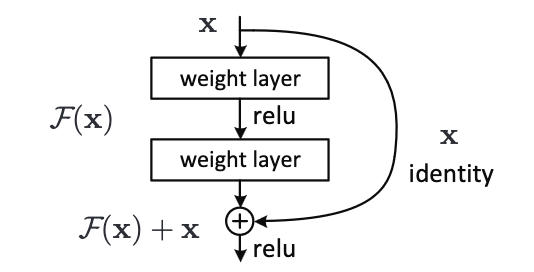
\includegraphics[width=13cm]{images/blackboxes/res_block.png}
\caption{Residual Block Diagram. Source \cite{resnet101}}
\end{figure}

The ResNet-101 architecture consists of 101 layers, including convolutional layers, pooling layers, and fully connected layers. The model employs a bottleneck structure in each residual block, reducing computational complexity while maintaining performance. The architecture has demonstrated impressive performance on various image recognition tasks, including the ImageNet Large-Scale Visual Recognition Challenge (ILSVRC) \cite{imageNet}, where it achieved state-of-the-art results.  With its ability to effectively train very deep models, ResNet-101 has contributed significantly to advancements in the field of deep learning and medical image analysis.

\begin{figure}
\centering
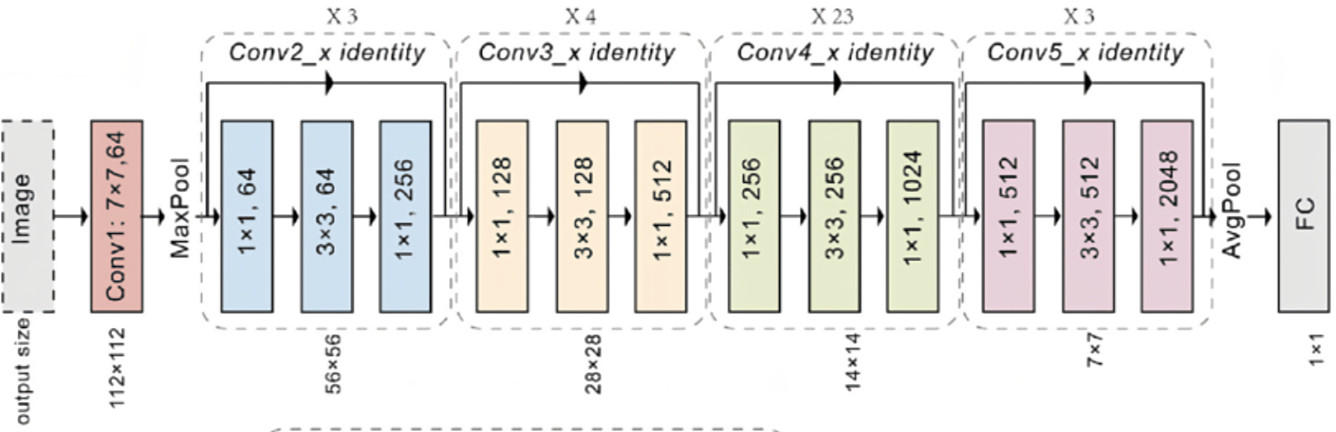
\includegraphics[width=13cm]{images/blackboxes/resnet101.png}
\caption{Resnet101 Architecture Diagram. Source \cite{resnet101Diagram}}
\end{figure}


\subsubsection{InceptionV3}
The InceptionV1 model addresses the problem of overfitting that arises when using deep layers of convolutions by employing parallel layers of multiple filter sizes at the same level. This wider architecture prevents the model from becoming excessively deep, mitigating overfitting risks.

\begin{figure}
\centering
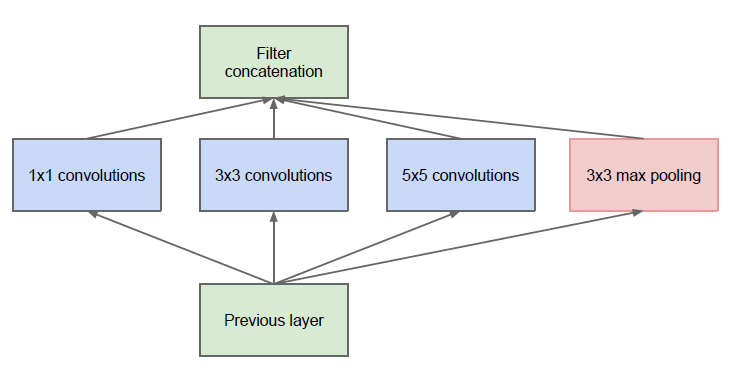
\includegraphics[width=13cm]{images/blackboxes/inception_module.png}
\caption{Naive Form of Inception Block. Source \cite{resnet101}}
\end{figure}

InceptionV3 further enhances the original Inception design with several modifications. One key modification is the factorization of the 5×5 convolutional layer into two 3$\times$3 convolutional layers, reducing computational costs while maintaining expressive power. Another improvement involves spatial factorization, replacing n×n convolutions with a 1×n convolution followed by an n×1 convolution. This two-layer solution reduces computational expenses by 33\% when the number of input and output filters is equal.

\begin{figure}
\centering
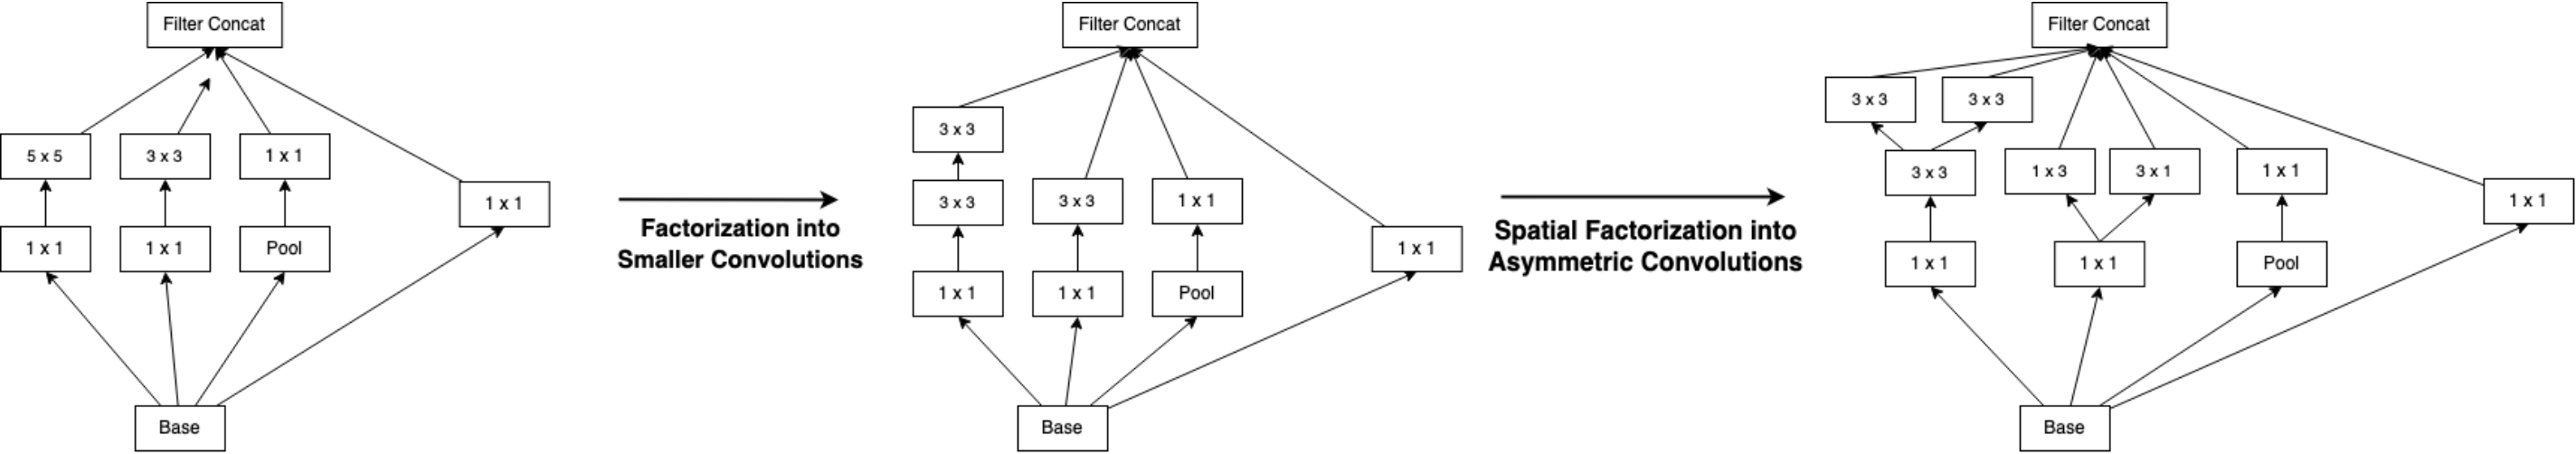
\includegraphics[width=13cm]{images/blackboxes/inception3_ideas.png}
\caption{Some major optimizations of InceptionV3 model. Source \cite{inceptionv3}}
\end{figure}

The InceptionV3 model also introduces the use of auxiliary classifiers, which act as regularization techniques for the architecture. These auxiliary classifiers aid in training by providing additional supervision during the learning process. Additionally, efficient grid size reduction is achieved through the utilization of two parallel blocks of convolution and pooling, which are later concatenated.

\begin{figure}
\centering
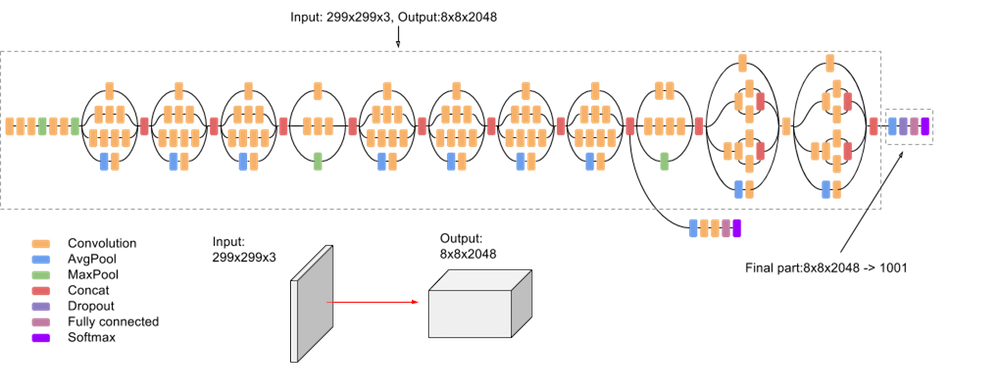
\includegraphics[width=13cm]{images/blackboxes/inceptionv3.png}
\caption{InceptionV3 Architecture. Source \cite{inceptionv3}}
\end{figure}

Another modification is the reduction in the grid size of feature maps by employing two parallel blocks of convolution and pooling. This design allows for a more efficient reduction in grid size while maintaining the expressive power of the network. Specifically, if we start with a $w\times w$ grid with $k$ filters, after reduction, it results in a $w/2\times w/2$ grid with $2k$ filters. By expanding the activation dimension in this manner, InceptionV3 ensures more efficient use of network capacity and computation. The two parallel blocks of convolution and pooling operate independently, capturing different types of information from the input. These blocks are then concatenated, combining the extracted features in a complementary way

These modifications in InceptionV3 enable improved performance and computational efficiency, making it a powerful model for various computer vision tasks. The Inception family of models has contributed significantly to the field of deep learning, demonstrating the effectiveness of wider architectures and factorization techniques in achieving state-of-the-art results.